% !TEX program = xelatex
% Normally Abnormal — print edition.
%
% Compile with XeLaTeX (on Overleaf: Menu → Compiler → XeLaTeX). The chapters in
% chapters/ and the charts in figures/ are generated from the website's .svx
% files by `npm run print`; edit the .svx, not those files. This file is yours:
% it is written once and never overwritten.

\documentclass[11pt,twoside,openright]{book}

% ——— Page: a 5.5 × 8.5 in trade page, as in the Verne edition ———
% The text width (5.5 − 0.85 − 0.675 = 3.975 in) is also set in
% scripts/print.mjs, which draws the charts at exactly that width.
\usepackage{geometry}
\geometry{
	papersize={5.5in,8.5in},
	top=0.925in,
	bottom=0.95in,
	inner=0.85in,
	outer=0.675in,
	headheight=14pt,
	headsep=0.2in,
	footskip=0.3in
}

% ——— Type: the website's faces ———
% EB Garamond for text, and Playfair Display (as "Abnormal Display": the font's
% licence reserves its name for unmodified copies, and these are static cuts of
% the variable font) for display type. Both are under the SIL Open Font License;
% see fonts/.
\usepackage{fontspec}
\setmainfont{EBGaramond}[
	Path=fonts/, Extension=.otf,
	UprightFont=*-Regular, ItalicFont=*-Italic,
	BoldFont=*-SemiBold, BoldItalicFont=*-SemiBoldItalic,
	Numbers={OldStyle,Proportional}
]
\newfontfamily\displayblack{AbnormalDisplay}[
	Path=fonts/, Extension=.ttf, UprightFont=*-Black, ItalicFont=*-BlackItalic, BoldFont=*-Black]
\newfontfamily\displaybold{AbnormalDisplay}[
	Path=fonts/, Extension=.ttf, UprightFont=*-Bold, ItalicFont=*-BoldItalic, BoldFont=*-Bold]
\newfontfamily\liningfigures{EBGaramond}[
	Path=fonts/, Extension=.otf, UprightFont=*-Regular, ItalicFont=*-Italic,
	BoldFont=*-SemiBold, Numbers={Lining,Monospaced}]

% Math: Garamond-Math where it is installed (it is on Overleaf), else Latin Modern.
\usepackage{amsmath}
\usepackage{unicode-math}
\IfFontExistsTF{Garamond-Math.otf}
	{\setmathfont{Garamond-Math.otf}[StylisticSet={7,9}]}
	{\setmathfont{Latin Modern Math}}

\usepackage{microtype}
\usepackage{setspace}
\setstretch{1.2}
\widowpenalty=10000
\clubpenalty=10000
\raggedbottom

% ——— Colour: the website's ink and oxblood ———
\usepackage{xcolor}
\definecolor{ink}{HTML}{26221C}
\definecolor{inksoft}{HTML}{4A443B}
\definecolor{inkfaded}{HTML}{7A7266}
\definecolor{oxblood}{HTML}{8E3B33}
\definecolor{ochre}{HTML}{A97C2C}
\color{ink}

% A small, letterspaced capital label: the book's "kicker" (Chapter One, Figure 2.4).
\newcommand{\kicker}[2][inkfaded]{%
	{\color{#1}\addfontfeatures{LetterSpace=14}\footnotesize\MakeUppercase{#2}}}

% Number words: Chapter One, Two, …
\newcommand{\numberword}[1]{\ifcase#1\or One\or Two\or Three\or Four\or Five\or Six\or
	Seven\or Eight\or Nine\or Ten\or Eleven\or Twelve\else #1\fi}

% The website's double rule: heavy over light.
\newcommand{\doublerule}[1][\linewidth]{%
	\par\noindent\rule{#1}{1.4pt}\par\vspace{-0.62\baselineskip}\noindent\rule{#1}{0.4pt}\par}

% ——— Chapters and sections ———
\setcounter{secnumdepth}{0} % chapters are numbered (figures are 2.1, 2.2, …); sections are not
\usepackage{titlesec}
\titleformat{\chapter}[display]
	{\centering}
	{\kicker{Chapter \numberword{\value{chapter}}}}
	{0.5em}
	{\displayblack\fontsize{24}{27}\selectfont}
	[\vspace{0.9em}\doublerule]
\titlespacing*{\chapter}{0pt}{0.45in}{0.35in}
\titleformat{\section}{\centering\displaybold\large}{}{0pt}{}
\titlespacing*{\section}{0pt}{1.7em plus 0.4em}{0.7em}
\titleformat{\subsection}{\centering\displaybold\normalsize}{}{0pt}{}
\titlespacing*{\subsection}{0pt}{1.3em plus 0.3em}{0.5em}

% ——— Contents ———
\usepackage{titletoc}
\titlecontents{chapter}[0pt]
	{\addvspace{0.9em}}
	{\parbox[t]{\linewidth}{\kicker{Chapter \numberword{\thecontentslabel}}}\\[0.15em]\displaybold}
	{\displaybold}
	{\nobreak\titlerule*[0.6pc]{.}\liningfigures\contentspage}
\setcounter{tocdepth}{0}

% ——— Running heads ———
\usepackage{emptypage} % blank left-hand pages carry no running head
\usepackage{fancyhdr}
\pagestyle{fancy}
\fancyhf{}
\fancyhead[LE]{\kicker{Normally Abnormal}}
\fancyhead[RO]{\kicker{\leftmark}}
\fancyfoot[LE,RO]{\liningfigures\small\thepage}
\renewcommand{\headrulewidth}{0pt}
\renewcommand{\chaptermark}[1]{\markboth{#1}{}}
\fancypagestyle{plain}{\fancyhf{}\fancyfoot[C]{\liningfigures\small\thepage}\renewcommand{\headrulewidth}{0pt}}

% ——— Drop caps ———
\usepackage{lettrine}
\renewcommand{\LettrineFontHook}{\displayblack}
\renewcommand{\LettrineTextFont}{\scshape}
\setcounter{DefaultLines}{3}
\setlength{\DefaultFindent}{2pt}
\setlength{\DefaultNindent}{0.3em}

% ——— Figures: kicker, title, chart, then source and note in small type ———
\usepackage{graphicx}
\usepackage{etoolbox}
\usepackage{caption}
\DeclareCaptionLabelFormat{kicker}{\kicker[oxblood]{#1~#2}}
\DeclareCaptionFont{display}{\displaybold\normalsize\setstretch{1.05}}
\captionsetup[figure]{
	position=top, labelformat=kicker, labelsep=newline,
	justification=raggedright, singlelinecheck=false,
	textfont=display, skip=5pt
}
% bookfigure: a float ruled like the website's figures, heavy above and light below.
\newenvironment{bookfigure}[1][htbp]
	{\begin{figure}[#1]\noindent\rule{\linewidth}{1.4pt}\par\vspace{3pt}}
	{\par\vspace{6pt}\noindent\rule{\linewidth}{0.4pt}\end{figure}}
% Tables: the same kicker, title and rules as figures ("Table 2.1").
\usepackage{booktabs}
\captionsetup[table]{
	position=top, labelformat=kicker, labelsep=newline,
	justification=raggedright, singlelinecheck=false,
	textfont=display, skip=5pt
}
\newenvironment{booktable}[1][htbp]
	{\begin{table}[#1]\noindent\rule{\linewidth}{1.4pt}\par\vspace{3pt}\small\liningfigures\setlength{\tabcolsep}{2pt}}
	{\par\vspace{6pt}\noindent\rule{\linewidth}{0.4pt}\end{table}}
\newcommand{\tablehead}[1]{{\color{inksoft}\addfontfeatures{LetterSpace=8}\scriptsize\MakeUppercase{#1}}}
% \figurenote{source}{note}: either may be empty.
\newcommand{\figurenote}[2]{%
	\ifblank{#1#2}{}{\par\vspace{4pt}{\scriptsize\setstretch{1.1}\raggedright\color{inksoft}%
		\ifblank{#1}{}{\kicker[inksoft]{Source}: #1. }%
		\ifblank{#2}{}{\textit{#2.}}\par}}}
\renewcommand{\topfraction}{0.92}
\renewcommand{\bottomfraction}{0.6}
\renewcommand{\textfraction}{0.06}
\renewcommand{\floatpagefraction}{0.75}
\setcounter{totalnumber}{2}

% ——— Field Guide cards ———
\usepackage{tikz}
\usepackage[most]{tcolorbox}
\newcounter{fieldguide}[chapter]
\renewcommand{\thefieldguide}{\thechapter.\arabic{fieldguide}}
\tcbset{
	guidecard/.style={
		enhanced, breakable, sharp corners,
		colback=white, colframe=ink, boxrule=0.6pt,
		borderline={0.4pt}{2.2pt}{ink},
		left=9pt, right=9pt, top=8pt, bottom=8pt,
		before skip=1.4em, after skip=1.6em,
		fontupper=\small\setstretch{1.12}
	}
}
% \begin{fieldguide}{Title}{label}
\newenvironment{fieldguide}[2]{%
	\refstepcounter{fieldguide}\label{#2}%
	\begin{tcolorbox}[guidecard]
	\kicker[oxblood]{Field Guide \thefieldguide}\par\vspace{1pt}
	{\displaybold\large\setstretch{1.05}#1\par}\vspace{4pt}
	{\color{ink}\hrule height 0.4pt}\vspace{6pt}%
}{\end{tcolorbox}}
% The applied card sits inside a figure, whose caption carries its title.
\newenvironment{appliedguide}{\begin{tcolorbox}[guidecard, breakable=false, before skip=2pt, after skip=0pt]}{\end{tcolorbox}}

\newcommand{\guidesection}[1]{\par\vspace{5pt}\noindent\kicker[inksoft]{#1}\par\vspace{3pt}}
\newcommand{\guidebox}[1]{\raisebox{-0.12em}{\tikz[line width=0.6pt,x=0.78em,y=0.78em]{\draw[ink] (0,0) rectangle (1,1); #1}}}
\newcommand{\guidecheck}[2]{\par\noindent\hangindent=1.4em\hangafter=1
	\makebox[1.4em][l]{\guidebox{}}\textbf{#1}\enspace #2\par\vspace{2pt}}
% \guideverdict{pass|partly|fail}{label}{reason}
\newcommand{\guidemark}[1]{%
	\ifstrequal{#1}{pass}{\guidebox{\draw[ink,line width=1pt,line cap=round] (0.2,0.52)--(0.42,0.25)--(0.82,0.8);}}{%
	\ifstrequal{#1}{fail}{\guidebox{\draw[oxblood,line width=1pt,line cap=round] (0.22,0.22)--(0.78,0.78) (0.22,0.78)--(0.78,0.22);}}{%
	\guidebox{\draw[ochre,line width=1.2pt,line cap=round] (0.25,0.5)--(0.75,0.5);}}}}
\newcommand{\guideword}[1]{%
	\ifstrequal{#1}{pass}{\kicker[ink]{Pass}}{\ifstrequal{#1}{fail}{\kicker[oxblood]{Fail}}{\kicker[ochre]{Partly}}}}
\newcommand{\guideverdict}[3]{\par\noindent\hangindent=1.4em\hangafter=1
	\makebox[1.4em][l]{\guidemark{#1}}\textbf{#2}\enspace\guideword{#1}\enspace #3\par\vspace{2pt}}
\newcommand{\guidepara}[1]{\par\vspace{6pt}\noindent #1\par}
% \guidestep{label}{text}: a numbered step, counting from 1 in each card.
\newcounter{guidestep}
\AtBeginEnvironment{fieldguide}{\setcounter{guidestep}{0}}
\newcommand{\guidestepnum}{\stepcounter{guidestep}\raisebox{-0.12em}{\tikz[line width=0.6pt,x=0.8em,y=0.8em]{%
	\draw[ink] (0.5,0.5) circle (0.55); \node[font=\scriptsize\liningfigures,inner sep=0] at (0.5,0.47) {\arabic{guidestep}};}}}
\newcommand{\guidestep}[2]{\par\noindent\hangindent=1.4em\hangafter=1
	\makebox[1.4em][l]{\guidestepnum}\textbf{#1}\enspace #2\par\vspace{2pt}}

% ——— Notes and links ———
\usepackage[hang,flushmargin]{footmisc}
\renewcommand{\footnotelayout}{\setstretch{1.05}}
\usepackage[hidelinks]{hyperref}

\begin{document}

\frontmatter
\pagestyle{empty}

% ——— Title page ———
\begin{titlepage}
	\centering
	\vspace*{1.3in}
	{\displayblack\fontsize{30}{32}\selectfont Normally\\[2pt]Abnormal\par}
	\vspace{0.9em}
	\doublerule[0.55\linewidth]
	\vspace{0.8em}
	{\itshape\large Why Real-World Data So Rarely\\Follow a Bell Curve\par}
	\vfill
	{\kicker[ink]{Matthew T. Helm}\par}
	\vspace{0.6in}
\end{titlepage}

% ——— Copyright page ———
\thispagestyle{empty}
\vspace*{\fill}
{\footnotesize\setstretch{1.15}\raggedright
\textit{Normally Abnormal: Why Real-World Data So Rarely Follow a Bell Curve}\\
Copyright © 2026 Matthew T. Helm. All rights reserved.\par\medskip
Draft edition, typeset \today.\par\medskip
The figures are drawn from public data; each lists its source.
Set in EB Garamond and Playfair Display, both under the SIL Open Font License.\par}
\cleardoublepage

\pagestyle{fancy}
\tableofcontents

\mainmatter
% Generated by scripts/print.mjs: every chapter, in order.
% The Average Millionaire — generated from src/chapters/01-average-millionaire/index.svx by scripts/print.mjs.
% Do not edit: changes here are overwritten on the next export.

\chapter{The Average Millionaire}
\label{ch:average-millionaire}

\section{Not So Average After All}

\lettrine[ante=“]{H}{ey,} Matt. You’re a data guy, right?” I shrugged and nodded at the same time, acknowledging that I \emph{am} a data guy, but I was reluctant to allow myself to be reduced to such a singular description. “What’s the average net worth of an American family?”

Having recently reviewed the Federal Reserve’s 2022 release of its \emph{Survey of Consumer Finances}, I responded, “The \emph{average} net worth was a little more than \$1 million in 2022, but…”

Before I could qualify my answer, Martin, a colleague with whom several others and I were having lunch, contorted his face into a look representing some mixture of confusion, disbelief, and apprehension as he exclaimed, “What!?! There’s no way that’s true!”

I calmly finished my statement by saying, “…the \emph{median} net worth was only about \$192,000.” Martin looked relieved. He was about five years away from retirement, and didn’t mind telling us that a rough estimate of his own net worth comfortably exceeded that figure.

“So, I’m above average! Not bad!” he declared.

“Well, actually…” Not wanting to come across as pedantic or fastidious, I left it there.

I’ve had many conversations like this over the course of my career as a data scientist, and I’ve found that people have a strong desire or need to summarize and compress information into a single value, particularly for purposes of comparison. It’s just easier to reason about a problem when we can compare \(x\) to \(y\) and see which one is larger or smaller. Our brains summarize automatically, and we can only hold a small handful of items in our short-term memory at any given moment in time. Psychologists once put the number at seven, give or take a couple, but the modern estimate is closer to just four.\footnote{George A. Miller, “The Magical Number Seven, Plus or Minus Two: Some Limits on Our Capacity for Processing Information,” \emph{Psychological Review} 63, no. 2 (1956): 81–97; Nelson Cowan, “The Magical Number 4 in Short-Term Memory: A Reconsideration of Mental Storage Capacity,” \emph{Behavioral and Brain Sciences} 24, no. 1 (2001): 87–114.} Either way, it’s not a lot. Given this constraint, it makes sense for us to condense information to make it easier work through a problem.

The trouble with this, and with Martin’s question, is that wealth is not normally distributed. The net worth distribution doesn’t conform to a nicely shaped, symmetrical bell curve with a single peak and few values that lie far from the center. In truth, around 7.5\% of families have negative net worth, most have a relatively small net worth, and a tiny fraction of American families are worth billions of dollars. If we plot an estimate of the wealth distribution for American families using the Fed’s 2022 data, as well as the average (mean) and median values, it looks like this:

\begin{bookfigure}
	\caption{Net Worth of U.S. Families, 2022}\label{fig:net-worth}
	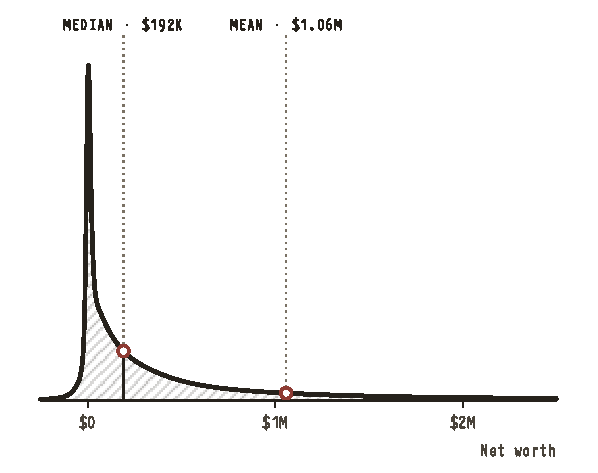
\includegraphics[width=\textwidth]{figures/1-1-net-worth.pdf}
	\figurenote{Federal Reserve, Survey of Consumer Finances, 2022}{Families worth more than \$2.5 million extend off the right edge}
\end{bookfigure}

The line in Figure~\ref{fig:net-worth} shows how common net worths near each value on the horizontal axis are. Another way to think about it is that the area under the curve between two points on the horizontal axis represents the share of families whose net worth lies within that range. We see a sharp peak, fairly close to the \$0 mark, and that the distribution extends outward to the right with a long tail. Notice that the horizontal axis doesn’t go beyond \$2.5 million, but in reality, the tail is much longer. The wealthiest family in the survey’s public data was worth approximately \$2.4 billion. To show that value on a chart with a linear scale in a book would require \emph{very} wide pages. In fact, if the distance from \$0 to the \$2.5 million mark measures four inches on your page, the \$2.4 billion mark would lie 320 feet away --- more than the length of a football field! Observe also that the difference between the median and the mean is around \$867,000. This shows the importance of not conflating the concepts of mean and median, as Martin did in the conversation above.

So what do we want to know, then, when we ask about the average? We are probably asking about what’s \emph{typical} or \emph{most common}, and that is sometimes very different from the statistical mean. Looking at the distribution of net worth in Figure~\ref{fig:net-worth}, many of us might believe some value close to the peak is most representative of an American family’s net worth. In that case, we might consider the \emph{mode} of the distribution, or the most frequently occurring value. In this case, the mode is just a few thousand dollars. This presents its own problem, though. About six out of every seven families have a net worth that exceeds the mode. Does it make sense to call it the most representative value when it sits below almost everyone?

This is precisely the challenge that arises when trying to characterize non-normally distributed data with a single summary statistic. Take a moment to think about the median and mean values in Figure~\ref{fig:net-worth}. Does either seem better suited than the other to characterize the \emph{typical} American family’s net worth?

Maybe the problem is that for certain distributions, the very idea of a characteristic, typical, usual, or common value simply doesn’t apply. What do we do in these cases? These questions and ideas, among others, are what we will explore in this book. Before we begin digging into these issues, however, let’s take a look at how normally distributed data arise, and why simple averages do a good job of summarizing them.

\section{True or False}

There are many processes that can be measured with a simple binary outcome: either true or false, yes or no, success or failure. Businesses market to customers via email campaigns and a customer either opens the email, or doesn’t. Website visitors either make a purchase, or they leave without buying anything. In quality control processes, a product passes a quality test, or it fails. Applications for credit are approved or they are denied. Soccer players (or footballers, depending on where you are in the world) taking penalty kicks either score, or they don’t.

Statisticians call these kinds of processes \emph{Bernoulli trials}, named after the great 17th-century Swiss mathematician, Jacob Bernoulli. If we record each success as a \(1\), and each failure as a \(0\), the average is nothing more than the proportion of successes, calculated by taking the sum and dividing it by the total number of trials. As the number of trials increases, that proportion settles toward the true probability of success, often represented as \(p\).

To see this in action, let’s consider a soccer player taking penalty kicks. As we’ve already established, each attempt is a Bernoulli trial and it results in either a goal being scored, or no goal. Let’s assume that the true, underlying probability of this player scoring on any given attempt is 75\%. In the top half of Figure~\ref{fig:kicks}, we see the running calculation of the player’s average, which we can call \(\hat{p}\) (pronounced \emph{p-hat}), and how it evolves as the number of penalty kicks taken increases. After the first three kicks, \(\hat{p}\) is 100\%, and then it slumps down to 62\% after 26 kicks before trending upwards toward \(p\) as the number of attempts increases. In the bottom half, we see how \(\hat{p}\) evolves over a much larger number of trials, and we can see that the average success rate stabilizes after a couple of hundred measurements and remains tantalizingly close to \(p\), the true probability of success.

Notice the gray-shaded region on the left-hand side of this plot. The average success rate is very unstable here and tends to swing dramatically as more attempts are added into the mix. This is a sample size effect. If we estimate the probability of success using a small sample, we end up with very different results. As sample sizes get bigger and bigger, our results begin to settle down and calculations from one large sample don’t differ much from the others. This is the \emph{law of large numbers} at work, and Bernoulli himself was the first to prove it. It’s responsible for \(\hat{p}\) gravitating toward \(p\).

\begin{bookfigure}
	\caption{The Share of Goals Settles Toward p}\label{fig:kicks}
	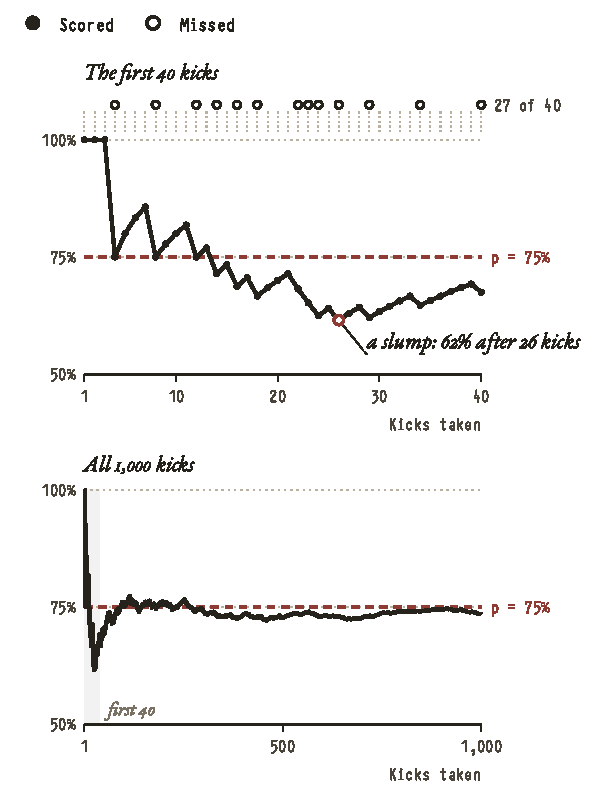
\includegraphics[width=\textwidth]{figures/1-2-kicks.pdf}
	\figurenote{Simulated}{1,000 penalty kicks by a player who scores 75\% of the time}
\end{bookfigure}

\section{Buckets of Success}

Suppose we take some number of penalty kick outcomes and put them into a bucket, the size of which we’ll just represent as \(n\). As we just established, the success rates for buckets with small \(n\) will tend to vary quite a bit more from bucket to bucket than those with large \(n\). With \(n = 1\), for example, there are only two possible values a bucket can have: 100\% or 0\%. If \(n = 2\), a bucket’s success rate can be 0\%, 50\%, or 100\%. As \(n\) increases, the number of possible success rates increases.

Consider the following experiment. We use buckets that contain either 1, 12, 40, or 100 kicks. For each bucket size, we use 10,000 separate buckets. In other words, we have 10,000 buckets that each contain a single penalty kick outcome, another 10,000 buckets that each contain the outcomes from a dozen kicks, and so on.

For our \(n = 1\) buckets (remember, each of these just tells us whether a single penalty kick resulted in a goal), we observe that 24.7\% of the kicks were unsuccessful and 75.3\% produced a goal. We see this in the top-left panel of Figure~\ref{fig:buckets}. There are two bars in this simple histogram, one for each outcome (either 0\% or 100\%) and the height of each bar corresponds to the percentage of the 10,000 buckets that yielded the corresponding outcome.

In the top-right panel, we have a similar plot, just with more bars since there are more possible outcomes with the larger bucket size of 12 kicks. In this plot, only 4\% of buckets had a success rate of 50\%, while the most common outcome (26.4\% of buckets) was a success rate of 75\%.

\begin{bookfigure}
	\caption{As Buckets Grow, the Shares Bunch Up Into a Bell}\label{fig:buckets}
	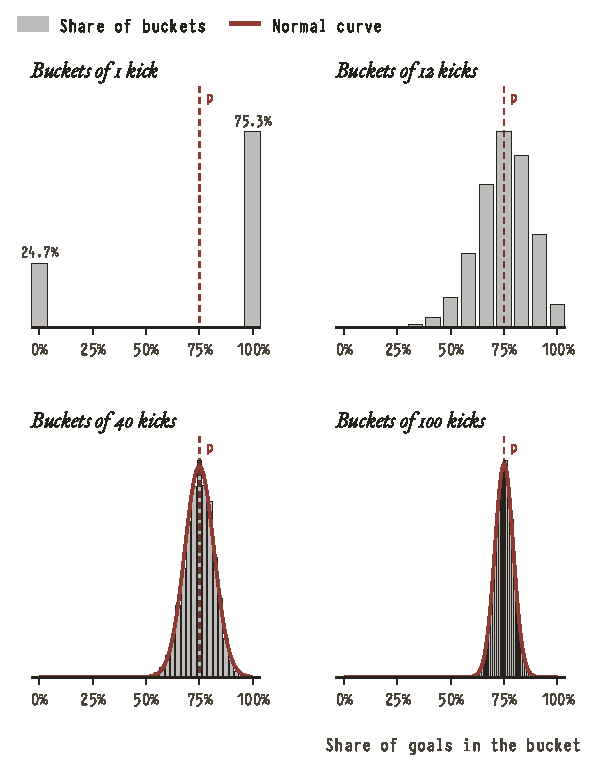
\includegraphics[width=\textwidth]{figures/1-3-buckets.pdf}
	\figurenote{Simulated}{10,000 buckets of each size; each panel has its own vertical scale}
\end{bookfigure}

Moving down to the bottom row, we see a very intriguing shape has emerged with our \(n = 40\) buckets. The largest share of the 10,000 buckets (15\%) had a success rate of 75\%, and all of our buckets tend to cluster around that figure, approaching a shape that looks like a normal distribution!

The final histogram calculated from the 10,000 buckets of 100 kicks each shows the same phenomenon as its bars conform to the smooth curve of the normal distribution even more closely.

So what does this mean? Can we summarize our soccer player’s penalty kick success rate (across many sets of 100 kicks) using a single number? We can, and Figure~\ref{fig:bell} shows why. It depicts a normal distribution of penalty kick success rates with a mean success rate of 75\% and a standard deviation of 4.3 percentage points. We haven’t discussed standard deviations yet, so for now, just think of the standard deviation as how spread out the distribution is. Large standard deviations yield shorter, wider distributions while smaller standard deviations produce taller, narrower distributions.

\begin{bookfigure}
	\caption{In a Normal Distribution, the Three Averages Agree}\label{fig:bell}
	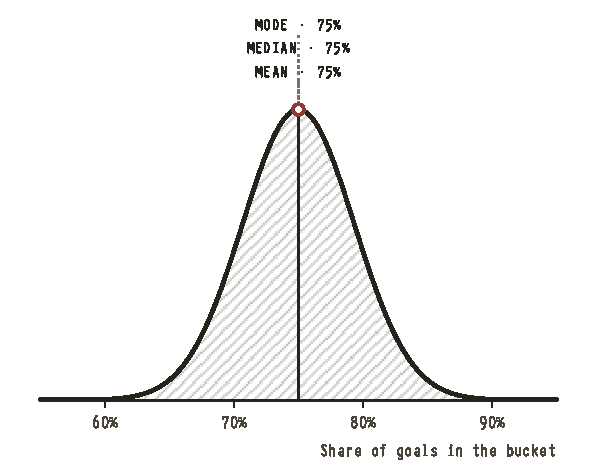
\includegraphics[width=\textwidth]{figures/1-4-bell.pdf}
	\figurenote{}{Normal curve for buckets of 100 kicks: mean 75\%, standard deviation 4.3 points}
\end{bookfigure}

This distribution shows us why it’s sometimes okay to use the word \emph{average} so loosely. Average is a slippery word, and people using it might be referring to the mean, median, or mode. When data are distributed normally, that’s completely acceptable --- they are in fact all the same value, as we see in Figure~\ref{fig:bell}.

\section{The Central Idea}

Let’s step back for a moment and briefly chronicle our journey from simple binary outcomes to a bell curve whose measures of central tendency (mean, median, and mode) are the same. In the top-left panel of Figure~\ref{fig:buckets}, we saw a histogram of single kick outcomes, and it looked nothing like a bell curve. However, once we started averaging over an increasing number of penalty kicks, those averages started bunching up into a bell shape.

This isn’t a peculiarity of penalty kicks --- it’s a mathematical result that statisticians call the \emph{Central Limit Theorem}. If you add up or average enough independent random pieces, the results tend toward a bell curve as you include more of them, almost regardless of what those individual pieces look like as long as certain conditions are met (note that computing a sum and an average are closely related; one is just divided by the count while the other is not). For example, consider the distribution of possible outcomes when rolling a die. For a single die, the distribution is flat, or uniform, across the discrete values of one to six. However, if you roll ten dice and take the sum, the distribution forms a bell curve (centered on 35 in this case). Another example might be a store’s daily sales total. The totals tend to form a bell curve, even though individual purchases are very uneven. A typical store might make many small sales in a day and just a few big sales, but because each day’s total is the sum of many purchases, the totals look like a normal distribution from one ordinary day to the next. Human heights are also approximately normally distributed, as they result from adding the effects of many genetic and environmental factors, each of which either increases or decreases an individual’s height relative to a baseline.

\section{The Fine Print}

At this point you may be slightly confused. This chapter opened with an example of data that are \emph{not} distributed normally, but we just saw that the bell curve arises when we take sums or averages of independent random variables, regardless of what they look like individually. So why didn’t it work with the net worth distribution?

Before we answer that, let me provide you with a checklist of sorts that we can use to determine whether we should expect a process to result in a normal distribution. A \emph{value} in the checklist is an aggregation of \emph{pieces.} For example, one bucket’s success rate is a \emph{value} built from individual penalty kicks, or \emph{pieces}.

\begin{fieldguide}{Should I Expect a Bell Curve?}{guide:bell-checklist}
	\guidesection{How each value is built}
	\guidecheck{Many pieces}{Does each value consist of many distinct pieces rather than a few?}
	\guidecheck{Additive}{Does each piece add to the total rather than multiplying it?}
	\guidecheck{Independent}{Is each piece roughly independent of the others, rather than driven by them?}
	\guidecheck{No giants}{Is every piece small relative to the total, so that no single piece can overwhelm the rest?}
	\guidesection{Whether the values belong together}
	\guidecheck{One group}{Do all the values come from one group as opposed to a mix of groups with different central tendencies?}
	\guidepara{\emph{All yes:} expect something close to a bell, with a single peak, a roughly symmetric shape, and few values far from the mean. \emph{Any no:} don’t count on a bell; it may warp, fracture, or never form at all.}
\end{fieldguide}

In the case of our penalty kick experiment with the \(n = 100\) buckets, we met the many pieces criterion (100 kicks per bucket), each piece was strictly additive (a single kick could only add zero or one to the total), our kicks were independent (we assume the result of one kick didn’t influence another), each piece was small (no penalty kick ever results in more than one goal), and they all came from a single player. This results in \emph{yes} answers to all of the questions in our checklist, and it’s why we saw the normal distribution emerge from the data.

Returning to our question about the net worth distribution, wealth fails several items on our checklist. Most importantly, it isn’t built by adding up many small pieces like our penalty kicks. Wealth grows through a multiplicative process, since returns compound and tomorrow’s gain depends on today’s value. This also touches on the independence test. Advantages tend to build on one another, so families that start with a large inheritance, for example, are more likely to build even more wealth over time. The Fed’s survey also mixes families at very different stages of life, from young couples who have only just begun to save to retirees near their lifetime peak, so the data fail our one-group test. In Chapter 2, we’ll look at a less extreme version of this with wage distributions, where we’ll explore these failures in more depth.

Our checklist in Field Guide 1.1 is intended to be concise, and it is not an exhaustive test that will work in every situation. However, I think it covers most of the cases that most readers will encounter in their daily lives, and it is therefore an incredibly useful tool. As you progress through the rest of the book, we’ll come back to it, and you should challenge yourself to work through it for the various data generating processes we will explore. This will help build a strong intuition for whether you can expect data to be normally distributed, which will in turn help you decide whether simple averages are sufficient for summarizing the data, or whether you will need to reach for other tools that you will acquire in later chapters.

\section{Crooked Averages}

So what happens when we compute an average for non-normal data? Assuming the arithmetic is performed accurately, you will end up with a number that is correct, at least mathematically. The issue is that the average is a summary, with strings attached, and those strings represent conditions that are often not met in the real world. When this occurs, the average, correct as it may be, simply isn’t telling you the whole story. Or even worse, it may even be telling you the \emph{wrong} story.

I stopped short of explaining these ideas to Martin because he seemed quite content to compare his own net worth to the median value, and it wasn’t the time or place to get into the weeds about the shape of the net worth distribution. However, you may now be able to imagine exactly what I would have told him. The net worth distribution is not normal, so one cannot safely conflate the concepts of mean, median, or mode. Martin declared that he was above average after learning that the \emph{median} value was roughly \$192,000. His net worth, accumulated over decades of (non-additive) compounding, is in fact \emph{below} average, but he’s in the top half of the net worth distribution, which is indeed a nice place to be.

In the rest of the book, we will explore a variety of distributions that, like the net worth distribution, are not normal. We will discover how to recognize data-generating processes that follow these non-normal distributions, and how to better characterize these data to make better decisions. In Chapter 2, in addition to wage distributions, we’ll look at house prices, which tend to be heavily skewed much like our net worth distribution from this chapter. We’ll see how the average compares to other statistics and how we can better tell the story of these distributions by simply looking at them from different perspectives.

% A Lopsided Victory — generated from src/chapters/02-lopsided/index.svx by scripts/print.mjs.
% Do not edit: changes here are overwritten on the next export.

\chapter{A Lopsided Victory}
\label{ch:lopsided}

\section{Show Me the Money}

\lettrine{I}{} once volunteered for a career day event at my daughter’s middle school. Like the other volunteers, my role was to occupy a seat at a table in the cafeteria, on top of which sat a sign with the name of my occupation, \emph{Data Scientist}, printed on it. Kids could stop by and talk to me about my profession and ask questions about what kinds of tasks it involves, what a typical day is like, and more. One young man, who seemed genuinely intrigued by my explanation of the work of a data scientist, seemed conflicted after our brief chat.

“I’ve always wanted to be a CEO, but your job \emph{does} sound really cool,” he remarked.

“What is it about being a CEO that appeals to you?” I asked.

“They get to be in charge, and they make a \emph{lot} of money!” he responded frankly. He didn’t know exactly how much he could expect to earn as a CEO, but he was sure that it was significantly more than most people who worked ordinary jobs.

For many people, expected earnings are a very important factor in deciding between careers or jobs. Wages, however, are not normally distributed, which creates challenges when comparing earnings statistics for two occupations. The Bureau of Labor Statistics regularly publishes wage data for standard occupational classifications, and if we use our checklist from Chapter 1, we can evaluate the process that generates these data and determine how likely they are to follow a bell curve.

First, an individual’s pay at a given point in time is shaped by dozens of factors, including their level of education, experience, geographic location, the industry in which they work, any licenses or specialized credentials they may hold, unique skills they may possess, and more. As a result, the process that generates wage data passes our \emph{many pieces} test.

The second test, for additivity, fails quite clearly. Pay raises are frequently calculated as a percentage, so a 4\% raise is worth far more in dollars to someone earning a high salary than to someone earning a lower one. Premiums for rare credentials or a particular geography, like a big city, also behave approximately like multipliers, and this again violates our second item on the checklist.

The independence test holds only partially. Workers with high levels of education are more likely to hold specialized credentials and licenses, high-paying industries are more likely to cluster in big cities, and rare skills are more likely to come with more experience. In essence, many of the pieces we outlined in the first test tend to move together, violating the requirement for independence. When this occurs, an individual’s advantages tend to accumulate rather than averaging out, which increases the spread across salary levels.

The \emph{no giants} test mostly passes, although occupations in which bonuses and commissions make up a large portion of a particular year’s pay may violate this.

Finally, the one-group test partially fails since certain occupational categories are much more heterogeneous than others. For example, \emph{General and operations managers} is a broad occupational category that encompasses a fairly wide range of management jobs, while \emph{Data scientists} tends to be a much narrower classification.

Here’s what our completed checklist might look like for salary data by occupation:

\begin{bookfigure}
	\caption{Field Guide 1.1, Applied to Wages}\label{fig:wage-checklist}
	\begin{appliedguide}
		\guidesection{How each value is built}
		\guideverdict{pass}{Many pieces}{Education, experience, location, industry, credentials, and skills all shape pay.}
		\guideverdict{fail}{Additive}{Raises and pay premiums are percentages, so they multiply rather than add.}
		\guideverdict{partly}{Independent}{Education, credentials, location, and experience tend to travel together.}
		\guideverdict{partly}{No giants}{Mostly small pieces, but bonuses and commissions can dominate a year’s pay.}
		\guidesection{Whether the values belong together}
		\guideverdict{partly}{One group}{Broad job titles, like general and operations managers, mix very different jobs.}
		\guidepara{\emph{Verdict:} don’t expect a bell. Expect a curve that leans to the right, as in Figure~\ref{fig:salaries}.}
	\end{appliedguide}
\end{bookfigure}

The test that fails most clearly is the one for additivity, and when this particular test fails, it tends to stretch the distribution to one side. Understanding why is fairly straightforward if we conduct a simple thought experiment: imagine two individuals, each earning \$100,000 per year. If the first individual doubles their salary twice (doubling is \emph{multiplying} by two), they end up at \$400,000. If the second individual halves their salary twice (dividing by two is the same as multiplying by one-half), they end up at \$25,000. The process is bounded at zero for the poor worker whose salary keeps halving, but the sky’s the limit for the lucky one who keeps experiencing a doubling of their salary. This multiplicative process leads to right-skewed distributions with long tails, like the ones we see in Figure~\ref{fig:salaries}.

\begin{bookfigure}
	\caption{Managers Earn More on Average; Data Scientists Earn More Typically}\label{fig:salaries}
	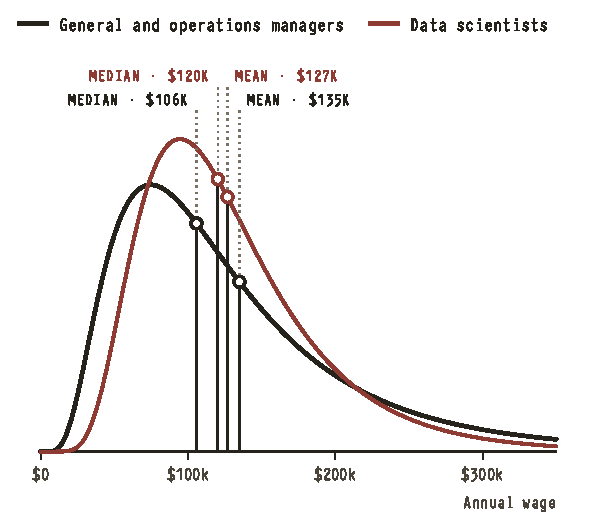
\includegraphics[width=\textwidth]{figures/2-2-salaries.pdf}
	\figurenote{Bureau of Labor Statistics, Occupational Employment and Wage Statistics, May 2025}{Curves are lognormal shapes fitted to each occupation’s published 25th and 75th percentile wages; each falls within about 5\% of the published 10th, 50th, and 90th percentiles and within about 2\% of the published mean. Markers show the published mean and median, colored by occupation}
\end{bookfigure}

In this figure we see two wage distributions: one for the \emph{General and operations managers} occupational category, and another for \emph{Data scientists.} While this particular class of managers is below the level that the young man from the career day event aspired to, it’s plausible that he may consider this occupational category some day. If he just looked at the mean salaries, he would conclude that workers in the manager classification earn more money than data scientists. However, the median values tell a different story. Half of all data scientists are estimated to earn at least \$120,000, while the corresponding figure for general and operations managers is just \$106,000.

\section{Playing the Game}

So which figure should we trust if our goal is to understand how much we can expect to earn in one occupation versus the other? Notice that the two lines in the plot cross at two points --- once around the \$73,000 mark, and again near \$214,000. We can think of our pay scale as being partitioned into three sections with the boundaries at those very points. Looking at it this way, we see that data scientist salaries are more concentrated in the middle section, while manager salaries are more concentrated at the ends. That is to say, managers are more likely to earn low salaries while also being more likely to earn very high salaries.

Comparing these kinds of distributions leaves the prospective worker in a situation that may feel somewhat like a game of chance. Imagine, for example, two booths at the county fair: at Booth A, everyone is guaranteed to win \$100, and at Booth B, there’s a 90\% chance you win \$95 and a 10\% chance that you win \$250. The average, or expected value, of Booth B’s winnings is \$110.50 (\(0.9 \times 95 + 0.1 \times 250\)) and the median payout is simply \$95. At Booth A, both the expected and median values are \$100. This means that Booth B will pay out more than Booth A \emph{on average}, but nine out of every ten players at Booth B will end up worse off than they would have been had they instead chosen to play at Booth A. However, the law of large numbers tells us that the average winnings of those who play at Booth B over and over again will eventually approach \$110.50. Nonetheless, that provides little comfort to someone choosing between careers because, as we all know, we only get to play the game of life once! In the case of our two wage distributions, the data scientist wage distribution is analogous to Booth A and general and operations managers are analogous to Booth B.

This exercise shows us that for certain distributions, comparisons require more nuance than simply checking a single measurement from each distribution. The larger mean combined with the lower median for the managers distribution provided a clue that it had a longer and fatter tail than that of the data scientists distribution, and the lower median from the managers distribution indicated that the typical manager earns less than the typical data scientist. Comparing the whole distributions made the picture very clear as it allowed us to see that managers’ salaries are spread out more than data scientists’ salaries.

We should also remind ourselves that salaries aren’t random --- for a student deciding on a career, their salary won’t be a random draw from the applicable salary distribution. Instead, it will be determined by the multitude of factors that we covered as we worked through the checklist. Even though a manager is more than twice as likely as a data scientist to earn less than \$60,000, that’s likely a result of the heterogeneity across the occupations within this particular occupational category. If the young man from the career day event obtains the right credentials and experience, and finds employment in a large city, for example, it would be reasonable for him to disregard the lower end of both of these distributions and instead focus on the higher end.

\section{Log Houses}

House prices are another example of a right-skewed distribution. Let’s once again work through our checklist to understand why this is the case:

\begin{bookfigure}
	\caption{Field Guide 1.1, Applied to Home Values}\label{fig:housing-checklist}
	\begin{appliedguide}
		\guidesection{How each value is built}
		\guideverdict{pass}{Many pieces}{Location, size, lot, age, condition, schools, and views all shape a home’s value.}
		\guideverdict{fail}{Additive}{Location and appreciation work as multipliers: the same house costs several times more in one city than another, and prices grow by percentages.}
		\guideverdict{partly}{Independent}{Big houses tend to be built on big lots, and condition is generally related to age.}
		\guideverdict{partly}{No giants}{In expensive cities, the land under a house can be worth more than the house itself.}
		\guidesection{Whether the values belong together}
		\guideverdict{fail}{One group}{Nationwide data mix housing markets as different as rural Mississippi and San Jose.}
		\guidepara{\emph{Verdict:} don’t expect a bell. Expect a curve with a long right tail, as in Figure~\ref{fig:home-values}.}
	\end{appliedguide}
\end{bookfigure}

The U.S. Census Bureau’s American Community Survey (ACS) is conducted annually and covers approximately 3.5 million addresses across the United States and Puerto Rico. Respondents are asked about where they live and what the value of their home is. Using the data for 2024, the mean home value for single-family, detached houses was \$501,000, the median was \$350,000, and the mode was \$268,000. This pattern, \(\text{mode} < \text{median} < \text{mean}\), tells us that we are dealing with a right-skewed distribution. Figure 2.4 shows an estimate of the probability density for home values, as reported by ACS respondents:

\begin{bookfigure}
	\caption{Home Values: A Long Tail to the Right}\label{fig:home-values}
	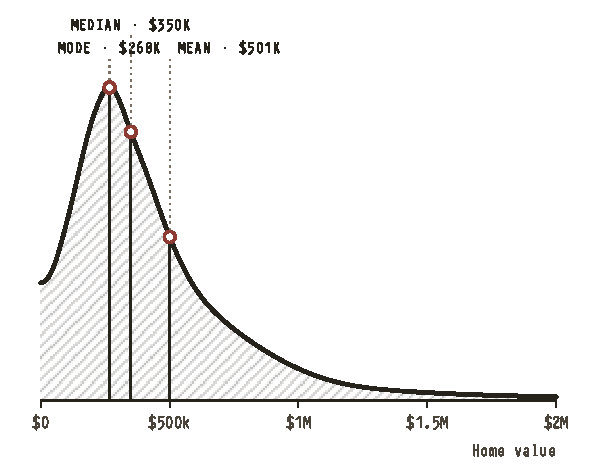
\includegraphics[width=\textwidth]{figures/2-4-home-values.pdf}
	\figurenote{U.S. Census Bureau, American Community Survey 1-year microdata, 2024}{Owner-occupied single-family detached homes, valued by their owners. About 2\% of homes are worth more than \$2 million and extend off the right edge}
\end{bookfigure}

We now know that the multiplicative effects of location and appreciation, at least in part, are responsible for the long tail we see in the plot. Just as we saw with the net worth distribution in Chapter 1, the horizontal axis in this plot is truncated because we are using a linear scale and cutting it short is necessary to produce a readable chart. However, if we simply change the scale of our x-axis, something very interesting happens, as you can see in Figure 2.5:

\begin{bookfigure}
	\caption{On a Log Scale, the Bell Comes Back (Mostly)}\label{fig:home-values-log}
	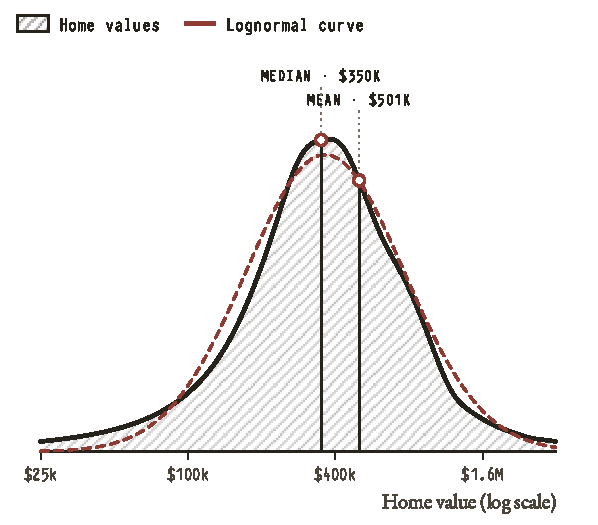
\includegraphics[width=\textwidth]{figures/2-5-home-values-log.pdf}
	\figurenote{U.S. Census Bureau, American Community Survey 1-year microdata, 2024}{Each step along the axis multiplies the value rather than adding to it. The dashed lognormal curve is fitted to the 25th and 75th percentiles. About 2\% of homes are worth less than \$25,000 and 1\% more than \$3.2 million}
\end{bookfigure}

By simply shifting from a linear scale to a logarithmic one, our home values data bunch up into a rough bell shape. Notice in Figure 2.4 that each increment on the x-axis is an increase in value of \$200,000, but in Figure 2.5, each increment represents a 4x increase in value --- this is the log transform in action. When a distribution forms a bell curve on a log scale, it is simply known as a \emph{lognormal} distribution, and many processes follow this kind of distribution. Everything from asset prices, incomes, and firm sizes, to rainfall, network response times, and viral loads have been shown to follow a lognormal distribution.

So how does this help us in practice? Let’s consider more home value data. This time, we’ll look at the distributions for two different states, and we’ll see how the log transformation, along with a few tweaks in how we think about and describe the data, helps us perform a better analysis.

Figure 2.6 shows estimates of the probability densities for home values in Wisconsin, compared to Massachusetts, again on a log scale.

\begin{bookfigure}
	\caption{Same Shape, Twice the Price}\label{fig:state-pair}
	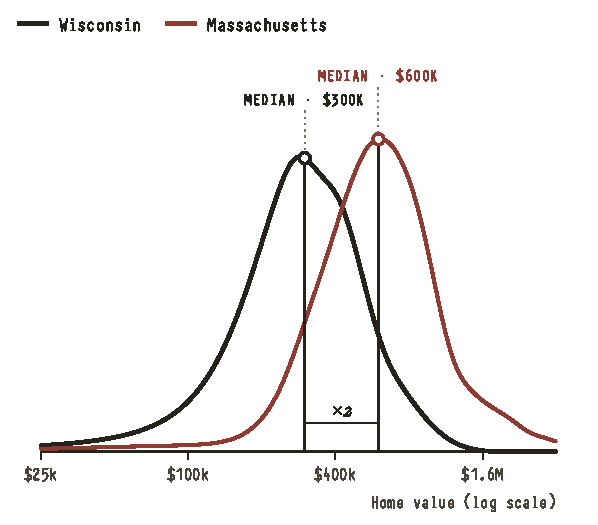
\includegraphics[width=\textwidth]{figures/2-6-state-pair.pdf}
	\figurenote{U.S. Census Bureau, American Community Survey 1-year microdata, 2024}{Owner-occupied single-family detached homes, valued by their owners. The Census Bureau reports the highest values in each state (just under 1\% of homes) only as above a cap, so the curves leave them out}
\end{bookfigure}

We can see from this plot that the shape of the distributions on the log scale is strikingly similar, just shifted. Remembering that our log axis is effectively a multiplicative scale, this allows us to compare the two markets with a single value, just stated as a multiple. In fact, home values in Massachusetts are roughly two times home values in Wisconsin, across their respective distributions. Table 2.1 demonstrates this:

\begin{booktable}
	\caption{Home Values in Wisconsin and Massachusetts}\label{tab:state-pair-table}
	\begin{tabular*}{\linewidth}{@{}l@{\extracolsep{\fill}}rrrrrr@{}}
		\toprule
		\tablehead{State} & \tablehead{10th} & \tablehead{25th} & \tablehead{Median} & \tablehead{75th} & \tablehead{90th} & \tablehead{Mean} \\
		\midrule
		Wisconsin & \$125K & \$200K & \$300K & \$420K & \$600K & \$350K \\
		Massachusetts & \$300K & \$415K & \$600K & \$850K & \$1.2M & \$740K \\
		\midrule
		\textit{Ratio} & \textit{2.4×} & \textit{2.1×} & \textit{2.0×} & \textit{2.0×} & \textit{2.0×} & \textit{2.1×} \\
		\bottomrule
	\end{tabular*}
	\figurenote{U.S. Census Bureau, American Community Survey 1-year microdata, 2024}{Percentiles and means of owner-reported values for owner-occupied single-family detached homes. The ratio is Massachusetts ÷ Wisconsin}
\end{booktable}



\end{document}
